\section{Architecture}\label{design}

Our analysis starts from the scenario illustrated in
Figure~\ref{fig:wasi}. Currently, WASI-compliant runtimes
implement dedicated user-space wrappers to enforce the
security boundaries of hostcalls. File system access is granted by the
user on a set of pre-opened directories that are specified via CLI
before the Wasm module is run (e.g., with the {\tt -{}-dir} option).
We follow a similar approach, asking the user to state the permissions
of each Wasm module in a JSON policy file. Contrary to existing
runtimes, permissions can be granted with file-based granularity.
Three permissions are available: (i) {\tt read} to open and read a
file, (ii) {\tt write} to modify, truncate and append content to a
file, and (iii) {\tt delete} to remove the file. When permissions are
related to a directory, {\tt read} translates to listing its content,
{\tt write} allows to create and delete files within it. We extended the Wasmtime
and WasmEdge runtimes to load the policy at startup, and, instead of
pre-opening the directories available to the Wasm module, we enforce
the policy with eBPF. eBPF code is split into programs attached to a
kernel- or user-space function called {\em hook point} and executed
whenever the hook is reached. Programs have visibility of function
parameters, they can persist state and share it with user space using
{\em maps}, and most of all they can enforce security checks based on
this information. Once the policy is encoded inside the map and the
eBPF programs are loaded, the runtime instantiates the
Wasm module selected by the user (arrow \blackcircle{A} in
Figure~\ref{fig:arch}). At this stage, the modified runtime invokes
a dedicated user probe specifying as a parameter the policy
that confines the loaded Wasm module~(\blackcircle{B}). The argument
is captured by a dedicated eBPF program that also annotates the
identifier of the thread running the Wasm interpreter in a tracing
map. We highlight that the policy is activated before the runtime
executes the module (i.e., before untrusted code is interpreted).
The consequence is that, from this point on, all the hostcalls
performed by the Wasm module are restricted by our eBPF programs
(arrows~\whitecircle{1}, ~\whitecircle{2}). The eBPF programs that make the
security decisions are evaluated every time a file-related kernel
security hook is reached (e.g., {\tt security\_file\_open}), and any
access decision is enforced at kernel level. When an unauthorized
request is performed by the Wasm code~(\whitecircle{3}), the related
eBPF program detects the violation and denies the request, returning
to the caller a permission denied error. When the execution of untrusted 
Wasm code terminates, another eBPF program is responsible for 
removing the access restriction from the thread executing the Wasm
runtime. No further intervention from the runtime is required, as the
maps and the eBPF programs are automatically removed from the kernel
immediately after the process running the runtime terminates.

This architecture offers several advantages. First, it eliminates the
risks coming from buggy user-space security checks (e.g., wrong
filepath resolution~\cite{parentfix}, wrong directory
removal~\cite{removedirfix}). Then, by leveraging kernel hook
points~\cite{bpf-lsm-hooks}, our approach allows the runtime developer
to focus on the interaction between Wasm code and the memory unsafe
system call, leaving aside authorizations and policy-related issues.
Lastly, access constraints can be audited by simply looking at the
JSON policy, instead of inspecting the code.

\begin{figure}[t!]
     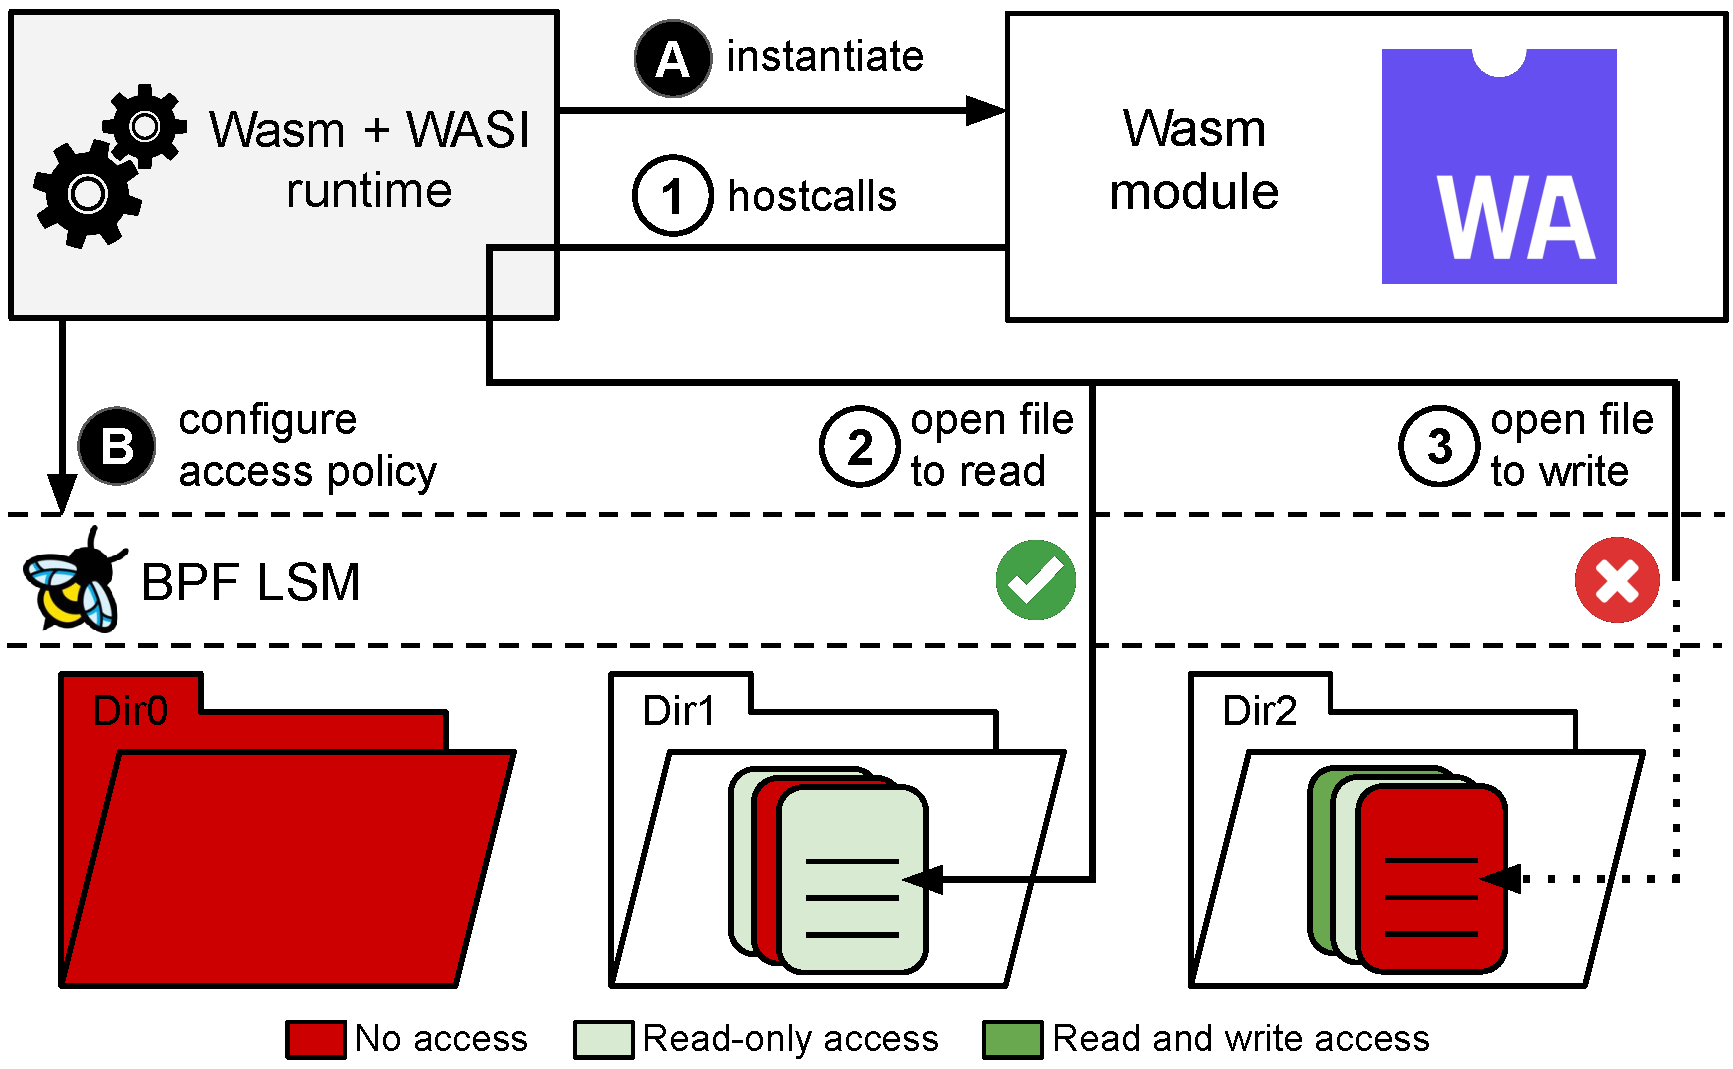
\includegraphics[width=\columnwidth]{chapters/wasm/fig/wasi-bpf}
     \caption[eBPF-based restriction of Wasm modules]{
          eBPF-based restriction of Wasm modules. The runtime
          instantiates the Wasm module (\blackcircle{A}), and
          configures the associated policy calling the traced user
          probe (\blackcircle{B}). After the Wasm module is run, all
          the hostcalls issued by the program (\whitecircle{1}) are
          restricted by eBPF (\whitecircle{2}, \whitecircle{3})
     }
     \label{fig:arch}
\end{figure}


%%% Local Variables:
%%% mode: latex
%%% TeX-master: "../main.tex"
%%% End:
